\documentclass[a4paper]{article}

\def\nbook {All of Statistics: A Concise Course in Statistical Inference}
\def\nbookshort {All of Statistics}

% Shared preamble. The fallback lets the document build whether the working
% directory is its own folder or the project root.
\IfFileExists{headerallofstats.tex}{\input{headerallofstats}}{%%%%%%%%%%%%%%%%%%%%
% AUTHOR AND HEADER
% define \nbook
%%%%%%%%%%%%%%%%%%%%

\makeatletter
\ifx \nauthor\undefined
  \def\nauthor{David A. Lee}
\else
\fi

\author{\nbook \\ \small Solutions by \nauthor}
\date{}

%%%%%%%%%%%%%%%%%%%%
% PACKAGES
%%%%%%%%%%%%%%%%%%%%

\usepackage{alltt} 
\usepackage{amsfonts}
\usepackage{amsmath}
\usepackage{amssymb}
\usepackage{amsthm}
\usepackage{bm}
\usepackage{booktabs}
\usepackage{caption}
\usepackage{centernot}
\usepackage{enumitem}
\usepackage{fancyhdr}
\usepackage[T1]{fontenc}
\usepackage{graphicx}
% Images live in chap1/ ... chap8/ at the project root, while the documents that
% use them sit one level down (allofstats/, allofstatschap1/, ...). Listing both
% "./" and "../" lets a document keep writing \includegraphics{chap1/foo.eps}
% and still resolve it whether it is compiled from its own folder or from the
% project root.
\graphicspath{{./}{../}}
\usepackage{mathdots}
\usepackage{mathtools}
\usepackage{microtype}
\usepackage{multirow}
\usepackage{pdflscape}
\usepackage{pgfplots}
\pgfplotsset{compat=1.18}
\usepackage{siunitx}
\usepackage{slashed}
\usepackage{tabularx}
\usepackage{tikz}
\usepackage{titletoc}
\usepackage{tkz-euclide}
\usepackage[normalem]{ulem}
\usepackage{url}
\usepackage[all]{xy}
\usepackage{imakeidx}

% fonts
% use \textsf to change to Computer Modern Bright
\renewcommand{\sfdefault}{cmbr} % keeps default font Computer Modern Roman

% makeindex for table of contents
\makeindex[intoc, title=Index]
\indexsetup{othercode={\lhead{ Index }}}

% table of contents remove numbering
\setcounter{secnumdepth}{0}

% pagestyle
\pagestyle{fancyplain}

% header
\lhead{	\nouppercase{\leftmark} }
\ifx \nextra \undefined
  \rhead{
    \ifnum\thepage=1
    \else
      \nbookshort \  | \nauthor
    \fi}
\else
  \rhead{
    \ifnum\thepage=1
    \else
      \nbookshort (\nextra)
    \fi}
\fi

% proof environment

\newcommand{\prooffont}{\scshape}
\usepackage{xpatch}
\tracingpatches
\xpatchcmd{\proof}{\itshape}{\prooffont}{}{}

% Python environment (for typesetting Python code)

% Default fixed font does not support bold face
\DeclareFixedFont{\ttb}{T1}{txtt}{bx}{n}{8} % for bold
\DeclareFixedFont{\ttm}{T1}{txtt}{m}{n}{8}  % for normal

% Custom colors
\usepackage{color}
\definecolor{deepblue}{rgb}{0,0,0.5}
\definecolor{deepred}{rgb}{0.6,0,0}
\definecolor{deepgreen}{rgb}{0,0.5,0}

\usepackage{listings}

% Python style for highlighting
\newcommand\pythonstyle{\lstset{
language=Python,
basicstyle=\ttm,
morekeywords={self},              % Add keywords here
keywordstyle=\ttb\color{deepblue},
emph={MyClass,__init__},          % Custom highlighting
emphstyle=\ttb\color{deepred},    % Custom highlighting style
stringstyle=\color{deepgreen},
frame=tb,                         % Any extra options here
showstringspaces=false
}}


% Python environment
\lstnewenvironment{python}[1][]
{
\pythonstyle
\lstset{#1}
}
{}

% Python for external files
\newcommand\pythonexternal[2][]{{
\pythonstyle
\lstinputlisting[#1]{#2}}}

% Python for inline
\newcommand\pythoninline[1]{{\pythonstyle\lstinline!#1!}}

%%%%%%%%%%%%%
% FUNCTIONS %
%%%%%%%%%%%%%

\DeclarePairedDelimiter\abs{\lvert}{\rvert}%
\DeclarePairedDelimiter\norm{\lVert}{\rVert}%

%%%%%%%%%%%%%%%%%%%%
% DOCUMENT GEOMETRY
%%%%%%%%%%%%%%%%%%%%

\ifx \ntrim \undefined
\else
  \usepackage{geometry}
  \geometry{
	  papersize={379pt, 699pt},
	  textwidth=345pt,
	  left=17pt,
	  top=54pt,
	  right=17pt,
  }
\fi

% maketitle statement
\title{}
\ifx \nisofficial \undefined
\let\@real@maketitle\maketitle
\renewcommand{\maketitle}{\@real@maketitle\begin{center}\begin{minipage}[c]{0.9\textwidth}\centering\footnotesize All errors, typographical and substantive, and other offenses, are entirely my own.\end{minipage}\end{center}}
\else
\fi

%%%%%%%%%%%%%%%%%%%%
% THEOREMS
%%%%%%%%%%%%%%%%%%%%

%\theoremstyle{definition}
\newtheorem*{axiom}{Axiom}
\newtheorem*{claim}{Claim}
\newtheorem*{conjecture}{Conjecture}
\newtheorem*{cor}{Corollary}
%\newtheorem*{dfn}{Definition}
\newtheorem*{eg}{Example}
\newtheorem*{ex}{Exercise}
%\newtheorem*{lemma}{Lemma}
\newtheorem*{prop}{Proposition}
%\newtheorem*{thm}{Theorem}
\newtheorem*{remark}{Remark}
\newtheorem*{warning}{Warning}

%%%%%%%%%%%%%%%%%%%%
% FORMATTING AESTHETICS
%%%%%%%%%%%%%%%%%%%%

% itemize bullets
\renewcommand{\labelitemi}{-}
\renewcommand{\labelitemii}{$\circ$}
\renewcommand{\labelenumi}{(\roman{*})}

% new page section
\let\stdsection\section
\renewcommand\section{\newpage\stdsection}

%%%%%%%%%%%%%%%%%%%%
% \mathbb commands
%%%%%%%%%%%%%%%%%%%%

\newcommand{\C}{\mathbb{C}}
\newcommand{\N}{\mathbb{N}}
\newcommand{\Q}{\mathbb{Q}}
\newcommand{\R}{\mathbb{R}}
\newcommand{\Z}{\mathbb{Z}}


%%%%%%%%%%%%%%%%%%%%
% Probability Operators
%%%%%%%%%%%%%%%%%%%%

\DeclareMathOperator{\Bernoulli}{Bernoulli}
\DeclareMathOperator{\betaD}{Beta}
\DeclareMathOperator{\bias}{\textsf{bias}}
\DeclareMathOperator{\binomial}{Binomial}
\DeclareMathOperator{\corr}{Corr}
\DeclareMathOperator{\cov}{\textsf{Cov}}
\DeclareMathOperator{\Exp}{Exp}
\DeclareMathOperator{\gammaD}{Gamma}
\DeclareMathOperator{\mse}{\textsf{MSE}}
\DeclareMathOperator{\multinomial}{Multinomial}
\DeclareMathOperator{\Poisson}{Poisson}
\DeclareMathOperator{\sd}{sd}
\DeclareMathOperator{\se}{\textsf{se}}
\DeclareMathOperator{\Uniform}{Uniform}
\newcommand{\Prob}{\mathbb{P}}
\newcommand{\var}{\mathbb{V}}
\newcommand{\E}{\mathbb{E}}

%%%%%%%%%%%%%%%%%%%%
% TCOLORBOX CODE FROM SeniorMars
%%%%%%%%%%%%%%%%%%%%

%\usepackage[varbb]{newpxmath} changes math font to newpxmath
\usepackage{xfrac}
\usepackage[makeroom]{cancel}
\usepackage{mathtools}
\usepackage{bookmark}
\usepackage{enumitem}
\usepackage{hyperref,theoremref}
\hypersetup{
	pdftitle={Assignment},
	colorlinks=true, linkcolor=doc!90,
	bookmarksnumbered=true,
	bookmarksopen=true
}
\usepackage[most,many,breakable]{tcolorbox}
\usepackage{xcolor}
\usepackage{varwidth}
\usepackage{varwidth}
\usepackage{etoolbox}
%\usepackage{authblk}
\usepackage{nameref}
\usepackage{multicol,array}
\usepackage{tikz-cd}
\usepackage[ruled,vlined,linesnumbered]{algorithm2e}
\usepackage{comment} % enables the use of multi-line comments (\ifx \fi)
\usepackage{import}
\usepackage{xifthen}
\usepackage{pdfpages}
\usepackage{transparent}

\newcommand\mycommfont[1]{\footnotesize\ttfamily\textcolor{blue}{#1}}
\SetCommentSty{mycommfont}
\newcommand{\incfig}[1]{%
    \def\svgwidth{\columnwidth}
    \import{./figures/}{#1.pdf_tex}
}

\usepackage{tikzsymbols}

% colors -- change them as you may!

\definecolor{myg}{RGB}{56, 140, 70}
\definecolor{myb}{RGB}{45, 111, 177}
\definecolor{myr}{RGB}{199, 68, 64}
\definecolor{mytheorembg}{HTML}{F2F2F9}
\definecolor{mytheoremfr}{HTML}{00007B}
\definecolor{mylenmabg}{HTML}{FFFAF8}
\definecolor{mylenmafr}{HTML}{983b0f}
\definecolor{mypropbg}{HTML}{f2fbfc}
\definecolor{mypropfr}{HTML}{191971}
\definecolor{myexamplebg}{HTML}{F2FBF8}
\definecolor{myexamplefr}{HTML}{88D6D1}
\definecolor{myexampleti}{HTML}{2A7F7F}
\definecolor{mydefinitbg}{HTML}{E5E5FF}
\definecolor{mydefinitfr}{HTML}{3F3FA3}
\definecolor{notesgreen}{RGB}{0,162,0}
\definecolor{myp}{RGB}{197, 92, 212}
\definecolor{mygr}{HTML}{880808}
\definecolor{myred}{RGB}{127,0,0}
\definecolor{myyellow}{RGB}{169,121,69}
\definecolor{myexercisebg}{HTML}{F2FBF8}
\definecolor{myexercisefg}{HTML}{88D6D1}
\definecolor{doc}{RGB}{0,60,110}

%================================
% THEOREM BOX
%================================

%\providecommand\theoremnumber{}
\tcbuselibrary{theorems,skins,hooks}
\newtcbtheorem{Theorem}{Theorem}
{%
	enhanced,
	breakable,
	colback = mytheorembg,
	frame hidden,
	boxrule = 0sp,
	borderline west = {2pt}{0pt}{mytheoremfr},
	sharp corners,
	detach title,
	before upper = \tcbtitle\par\smallskip,
	coltitle = mytheoremfr,
	fonttitle = \bfseries\sffamily,
	description font = \mdseries,
	separator sign none,
	segmentation style={solid, mytheoremfr},
}
{th}


%================================
% Question BOX
%================================

\makeatletter
\newtcbtheorem{question}{Question}{enhanced,
	breakable,
	colback=white,
	colframe=mygr,
	attach boxed title to top left={yshift*=-\tcboxedtitleheight},
	fonttitle=\bfseries\sffamily,
	title={#2},
	boxed title size=title,
	boxed title style={%
			sharp corners,
			rounded corners=northwest,
			colback=tcbcolframe,
			boxrule=0pt,
		},
	underlay boxed title={%
			\path[fill=tcbcolframe] (title.south west)--(title.south east)
			to[out=0, in=180] ([xshift=5mm]title.east)--
			(title.center-|frame.east)
			[rounded corners=\kvtcb@arc] |-
			(frame.north) -| cycle;
		},
	#1
}{def}
\makeatother

%================================
% PROPERTIES BOX
%================================

\tcbuselibrary{theorems,skins,hooks}
\newtcbtheorem{Property}{Property}
{%
	enhanced,
	breakable,
	colback = mytheorembg,
	frame hidden,
	boxrule = 0sp,
	borderline west = {2pt}{0pt}{mytheoremfr},
	sharp corners,
	detach title,
	before upper = \tcbtitle\par\smallskip,
	coltitle = mytheoremfr,
	fonttitle = \bfseries\sffamily,
	description font = \mdseries,
	separator sign none,
	segmentation style={solid, mytheoremfr},
}
{th}

%================================
% LEMMA
%================================

\tcbuselibrary{theorems,skins,hooks}
\newtcbtheorem[number within=section]{Lemma}{Lemma}
{%
	enhanced,
	breakable,
	colback = mylenmabg,
	frame hidden,
	boxrule = 0sp,
	borderline west = {2pt}{0pt}{mylenmafr},
	sharp corners,
	detach title,
	before upper = \tcbtitle\par\smallskip,
	coltitle = mylenmafr,
	fonttitle = \bfseries\sffamily,
	description font = \mdseries,
	separator sign none,
	segmentation style={solid, mylenmafr},
}
{th}


% Commands for special boxes
\newcommand{\thm}[2]{\begin{Theorem*}{#1}{}#2\end{Theorem*}}
\newcommand{\qs}[2]{\begin{question*}{#1}{}#2\end{question*}}
\newcommand{\prp}[2]{\begin{Property*}{#1}{}#2\end{Property*}}
\newcommand{\lemma}[2]{\begin{Lemma*}{#1}{}#2\end{Lemma*}}
}

\begin{document}
\maketitle

\section{Chapter 1: Probability}

\subsection*{Import Packages}

Please see the associated GitHub repo for all code and comments to simulations. [LINK HERE]

% QUESTION 1
\qs{1.10.1}{\textsf{Fill in the details of the proof of Theorem 1.8. Also, prove the monotone decreasing case.}}
\thm{(Wasserman 1.8) (Continuity of Probabilities)}{If \(A_{n} \rightarrow A\) then 
\[
	\Prob(A_{n}) \rightarrow \Prob(A)
\]
as \(n \rightarrow \infty\). 
}

\begin{proof}[Proof]
\textbf{Monotone Increasing Case.}
The intuition we exploit here is that monotonicity alone does not allow us to employ Kolmogorov Axiom 3. Therefore, we need to rewrite the monotone \(A\)'s in such a manner that the union of rewritten sets is disjoint.

Let $A_n$ be monotone increasing. By definition, $A_1 \subset A_2 \subset \cdots$. Let $A = \lim_{n \to \infty} A_{n} = \bigcup_{i=1}^{\infty} A_{i}$ and $B_{1} = A_{1}, B_{2} = \left\{\, \omega \in \Omega \colon \omega \in A_{2}, \omega \notin A_{1}  \,\right\}$, and so on. Take any $B_{i}, B_{j}$, with $i < j$. Our intuition here is that each $B_{i}$ consists of the ``new" $\omega$ that is ``added" to the previous $A_{i-1}$ to create the new $A_{i}$.
\begin{center}
	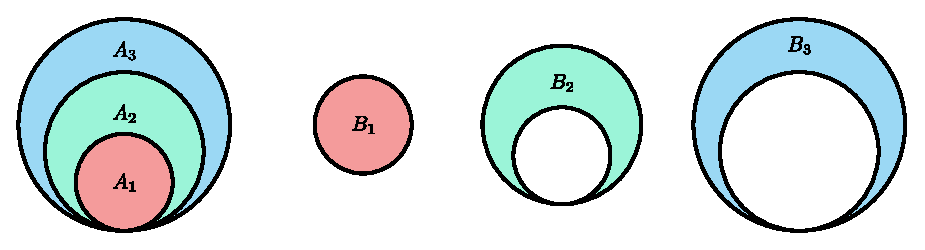
\includegraphics[width=\textwidth]{chap1/c1q1.eps}
\end{center}
Now, let \(\omega \in B_{i}\). We must have \(\omega \notin B_{j}\), since \(\omega \notin B_{i}\) is a condition for membership in \(B_{j}\). Thus \(B_{i} \cap B_{j} = \varnothing \), and each of the \(B\)'s are pairwise disjoint. 
Since \(A_{1} \subset \cdots \subset A_{n}\), we have
\[
	A_{n} = \bigcup_{i=1}^{n} A_{i} 
\]
Now consider \(\bigcup_{i=1}^{n} A_{i} \). Let \(\omega \in A_{n}\). Then \(\omega \in B_{n}\) implies \(\omega \in \bigcup_{i=1}^{n} B_{n} \). Conversely, let \(\omega \in \bigcup_{i=1}^{n} B_{n} \). Then \(\omega \in B_{i}\) for some \(i\), meaning we must have \(\omega \in A_{i}\); with \(A_{i} \subset A_{n}\), we must have \(\omega \in A_{n}\). Ergo, \(A_{n} = \bigcup_{i=1}^{n} B_{n}\).

We now have established
\[
	A_{n} = \bigcup_{i=1}^{n} A_{n} = \bigcup_{i=1}^{n} B_{n}
\]
and can conclude
\[
	\lim_{n \to \infty} A_{n} = \lim_{n \to \infty} \bigcup_{i=1}^{n} A_{n} = \lim_{n \to \infty} \bigcup_{i=1}^{n} B_{n} = A    
\]
By Kolmogorov Axiom 3 and the disjointness of the \(B\)'s, it follows that
\[
	P(A_{n}) = P\left( \bigcup_{i=1}^{n} B_{i}  \right) = \sum_{i=1}^{n} P(B_{i})	
\]
leaving the final step of taking the limits
\[
	\lim_{n \to \infty} P(A_{n}) = \lim_{n \to \infty} \sum_{i=1}^n P(B_{i}) = \sum_{i=1}^{\infty} P(B_{i}) =  P\left( \bigcup_{i=1}^{\infty} B_{i}  \right) = P(A)
\]
\textbf{Monotone Decreasing Case.} With \(A_{n}\) monotone decreasing so that \(A_{1} \supset A_{2} \supset \cdots \), let \(A = \lim_{n \to \infty} A_{n} = \bigcap_{i=1}^{\infty} A_{i}  \). By de Morgan's laws, we have
\[
	\left( \bigcap_{i=1}^{\infty} A_{i} \right)^{c} = \bigcup_{i=1}^{\infty} A_{i}^{c} 
\]
and when applied to the monotone increasing case,
\[
	\lim_{n \to \infty} P(A_{n}^{c}) = 1 - \lim_{n \to \infty} P(A_{n}) =  P \left( \bigcup_{i=1}^{\infty} A_{i}^{c} \right) = P(A^{c}) = 1 - P(A)  
\]

we can conclude
\[
	1 - \lim_{n \to \infty} P(A_{n}) = 1 - P(A) \implies \lim_{n \to \infty} P(A_{n}) = P(A) 
\]
\end{proof}

% QUESTION 2
\newpage
\qs{1.10.2}{Prove the statements in equation 1.1.}
\prp{(Wasserman Eq. 1.1)}{
	\begin{center}
	\begin{tabular}{r c l}
	$\Prob(\varnothing)$  &$=$ &$0$ \\
	$A \subset B$ &$\implies$ &$\Prob(A) \le \Prob(B)$ \\
	$0 \le$ &$\Prob(A)$ &$\le 1$ \\
	$\Prob(A^{c})$ &$=$ &$1 - \Prob(A)$ \\
	$A \bigcap B = \varnothing$ &$\implies$ &$P \big( A \bigcup B \big) = \Prob(A) + \Prob(B)$  
	\end{tabular}
	\end{center}}
\begin{proof}[Proof]
Let \(A, B\) be events. \\
\underline{$\Prob(\varnothing) = 0$} \\
We know that $\Omega^{c} = \varnothing$. Then $\Omega^{c} \cap \Omega = \varnothing$ and $\Omega^{c} \cup \Omega = \Omega$. Combining Kolmogorov Axioms 2 and 3, conclude $\Prob(\Omega) = \Prob(\Omega^{c}) + \Prob(\Omega) = \Prob(\varnothing) + \Prob(\Omega) = 1$. Another application of Axiom 2 yields $\Prob(\varnothing) = 1 - \Prob(\Omega) = 1 - 1 = 0$.

\underline{$A \subset B \implies \Prob(A) \le \Prob(B)$} \\
Consider \(A\) and \(B-A\). We have \(A \cap B-A = \varnothing\), as \(\omega \in A\) implies \(\omega \not\in B-A\) and \(\omega \in B-A\) implies \(\omega \not\in A\). 

Now we prove \(B = A \cup B-A\). If \(\omega \in A \cup B-A\) either \(\omega \in A\) or \(\omega \in B-A\). If \(\omega \in A\), then since \(A \subset B\), we have \(\omega \in B\). If \(\omega \in B-A\), then \(\omega \in B\). And if \(\omega \in B\), then \(\omega \in B-A\) implies \(\omega \in A \cup B-A\). Thus \(B = A \cup B-A\).

By Axiom 3,
\[
	\Prob(B) = \Prob(A \cup B-A) = \Prob(A) + \Prob(B-A)
\]
since \(\Prob(B-A) \ge 0\), this implies \(\Prob(A) \le \Prob(B)\).

\underline{\(0 \le \Prob(A) \le 1\)} \\
By Axiom 1, \(\Prob(A) \ge 0\). By Axioms 2 and 3, \(\Prob(\Omega) = 1 \). Then \(\Omega = A \cup A^{c}\) and \(A \cap A^{c} = \varnothing\), which in turn implies \(\Prob(\Omega) = \Prob(A) + \Prob(A^{c}) = 1\). Since \(\Prob(A^{c}) \ge 0\), we have \(\Prob(A) \le 1\). Thus \(0 \le \Prob(A) \le 1\).

\underline{\(\Prob(A^{c}) = 1 - \Prob(A)\)} \\
Since \(A^{c} \cap A = \varnothing\) and \(A^{c} \cup A = \Omega\), by Axioms 2 and 3, we have \(\Prob(\Omega) = 1 = \Prob(A) + \Prob(A^{c})\). We conclude that \(\Prob(A^{c}) = 1 - \Prob(A)\).

\underline{\(A \cap B = \varnothing \implies \Prob(A \cup B) = \Prob(A) + \Prob(B)\)} \\
By disjointness of \(A,B\), by Axiom 3, \(\Prob(A \cup B) = \Prob(A) + \Prob(B)\).
\end{proof}

\newpage
% QUESTION 3
\qs{1.10.3}{Let \(\Omega\) be a sample space and let \(A_{1}, A_{2}, \dots,\) be events. Define \(B_{n} = \bigcup_{i= n}^{\infty} A_{i} \) and \(C_{n} = \bigcap_{i=n}^{\infty} A_{i} \).
	\begin{enumerate}[label=(\alph*)]
		\item Show that \(B_{1} \supset B_{2} \supset \cdots\) and that \(C_{1} \subset C_{2} \subset \cdots\).
		\item Show that \(\omega \in \bigcap_{n=1}^{\infty} B_{n}\) if and only if \(\omega\) belongs to an infinite number of the events \(A_{1}, A_{2}, \dots\).
		\item Show that \(\omega \in \bigcup_{n=1}^{\infty} C_{n}\) if and only if \(\omega\) belongs to all the events \(A_{1}, A_{2}, \dots\) except possibly a finite number of those events.
	\end{enumerate}
}
\begin{proof}[Proof] 
	(a) For the base case, we prove \(B_{1} \supset B_{2}\). If \(\omega \in  B_{2} = \bigcup_{i=2}^{\infty} A_{i} \), then \(\omega \in A_{1} \cup \bigcup_{i=2}^{\infty} A_{i} = B_{1}\). Thus \(B_{1} \supset B_{2}.\)

Now assume \(B_{1} \supset \cdots \supset B_{n} \) is true. We want to prove that \(B_{1} \supset \cdots \supset B_{n} \supset B_{n+1}\). It will suffice to show \(B_{n} \supset B_{n+1}\). If \(\omega \in B_{n+1} = \bigcup_{i = n+1}^{\infty} A_{i} \), then we have \(\omega \in  A_{n} \cup \bigcup_{i = n+1}^{\infty} A_{i} = B_{n} \), so \(B_{n} \supset B_{n+1}\).

The proof for the \(C_{n}\)'s is analogous. For the base case, \(C_{1} \subset C_{2}\), if \(\omega \in C_{1} = \bigcap_{i=1}^{\infty} A_{i} \) then \(\omega \in A_{i}\) for all \(i\). Then we must have \(\omega \in A_{2}, A_{3}, \dots\), and consequently, \(\omega \in C_{2} = \bigcap_{i=2}^{\infty} A_{2} \).

For the induction hypothesis, suppose that \(C_{1} \subset \cdots \subset C_{n}	\). We must show \(C_{n} \subset C_{n+1}\). If \(\omega \in C_{n} = \bigcap_{i=n}^{\infty} A_{i} \), then we have \(\omega \in A_{n+1},\dots\) implying \(\omega \in C_{n+1} = \bigcap_{i=n+1}^{\infty} A_{n} \).
\vspace{12pt}
\par (b) \((\implies)\) Let \(\omega \in \bigcap_{n=1}^{\infty} B_{n} \). Suppose \(\omega\) belongs only to a finite number of events \(A_{i}\). Pick the \(A_{i}\) with the highest subscript \(i\). Now consider \(B_{i+1} = \bigcup_{j = i+1}^{\infty} A_{j} \). Our assumption of finitude implies \(\omega \not\in B_{i+1}\), a contradiction. We will come to this contradiciton for any choice of \(A_{i}\). Thus it must be that \(\omega\) belogns to an infinite number of events \(A_{i}\).

\(( \impliedby )\) Now suppose \(\omega\) belongs to an infinite number of events \(A_{i}\). We must show that \(\omega \in \bigcap_{n=1}^{\infty} B_{n}\).

For \(n=1\), we must have \(\omega \in  B_{1}\), as \(\omega\) is in infinitely many \(A_{i}\)'s, and \(B_{1} = \bigcup_{i=1}^{\infty} A_{i} \). 

Now suppose \(\omega \in B_{n} = \bigcup_{i=n}^{\infty} A_{i}\). To demonstrate \(\omega \in B_{n+1}\), we realize that we cannot have only \(\omega \in A_{n}, \omega \not\in A_{n+1}\), \dots as this would contradict the infinitude of membership. Thus we must have membership in \(A_{i}\)'s with \(i > n\). Ergo, \(\omega \in B_{n+1}\).

By induction, \(\omega \in B_{i}\) for all \(i\). Thus \(\omega \in \bigcap_{n=1}^{\infty} B_{n} \). 
\vspace{12pt}
\par (c) \(( \implies ) \) Let \(\omega \in \bigcup_{n=1}^{\infty} C_{n} \). Then \(\omega \in C_{n} = \bigcap_{i=n}^{\infty} A_{i} \) for at least one \(n\). If \(\omega \in C_{1} = \bigcap_{i=1}^{\infty} A_{i} \), then \(\omega\) belongs to all events \(A_{1}, A_{2},\dots\). Suppose otherwise that \(\omega \in  C_{n}\) for \(n \neq 1 \). Then \(\omega\) lacks membership in at least one of the \(A_{1},\dots, A_{n+1}\); in other words, it lacks membership in a finite number of those events.

\(( \impliedby )\) Let \(\omega\) belong to all \(A_{1}, A_{2}, \dots\) or otherwise lack membership in a finite number of \(A_{i}\). In the first case, \(\omega \in \bigcap_{i=1}^{\infty} A_{i} = C_{1} \) implies \(\omega \in \bigcup_{n=1}^{\infty} C_{n} \). Otherwise, pick the \(A_{i}\) with \(\omega \not\in A_{i}\) and the highest \(i\). Then we have \(\omega \in \bigcap_{j = i+1}^{\infty} A_{j} = C_{i+1} \), and still \(\omega \in \bigcup_{n = i+1}^{\infty} C_{n} \).
\end{proof}

% QUESTION 4
\qs{1.10.4}{Let \(\left\{\, A_{i} \colon i \in I \,\right\}\) be a collection of events where \(I\) is an arbitrary index set. Show that
\[
	\left( \bigcup_{i \in  I} A_{i}  \right)^{c} = \bigcap_{i \in  I} A_{i}^{c} \quad \text{and} \quad \left(\bigcap_{i \in I} A_{i} \right)^{c} = \bigcup_{i \in  I} A_{i}^{c} 
\]
Hint: First prove this for \(I = \{1, \dots, n \}\).
}

\begin{proof}[Proof]
These are the famous De Morgan's Laws.
\vspace{12pt}
\par (1) Let \(\omega \in \big(\bigcup_{i \in  I} A_{i} \big)^{c} \). Suppose \(I = \{1, \dots, n \} \). Then we have \(\omega \not\in \bigcup_{i \in  I} A_{i}\), with the following chain of implications: \(\omega \not\in A_{1}, \dots, A_{n}\) to \(\omega \in A_{1}^{c}, \dots, A_{n}^{c}\) to \(\omega \in \bigcap_{i \in  I} A_{i}^{c}\). Conversely, if \(\omega \in \bigcap_{i \in  I} A_{i}^{c}\), we must have \(\omega \not\in A_{1},\dots, A_{n}\), implying \(\omega \not\in \bigcup_{i \in  I} A_{i}\), allowing us to conclude \(\omega \in \big(\bigcup_{i \in  I} A_{i} \big)^{c} \).

That is the finite case. Suppose now that we prove the infinite case. In the base case, trivially \(\omega \in A_{1}^{c}\) implies itself. If we assume it holds for \(n-1 \  A_{i}\)'s, apply the proof for the \(n \  A_{i}\)'s to prove the infinite case by induction.
\vspace{12pt}
\par (2) Let \(\omega \in \big(\bigcap_{i \in  I} A_{i} \big)^{c}\) for \(i \in \{1, \dots, n \} \). Then \(\omega \not\in \bigcap_{i \in  I} A_{i}\), meaning \(\omega\) is bereft of membership for at least one \(A_{i}\). It follows that \(\omega \in A_{i}^{c}\), implying \(\omega \in \bigcup_{i \in  I} A_{i}^{c}\). Now suppose \(\omega \in \bigcup_{i \in  I} A_{i}^{c}\). Then \(\omega \in A_{i}^{c}\) for at least one \(i\). If so, we cannot have \(\omega \in \bigcap_{i \in  I} A_{i}\), so it must follow that \(\omega \in \big(\bigcap_{i \in  I} A_{i} \big)^{c}\). Thus \( \big(\bigcap_{i \in  I} A_{i} \big)^{c} = \bigcup_{i \in  I} A_{i}^{c}\).
\end{proof}

% QUESTION 5
\qs{1.10.5}{Suppose we toss a fair coin until we get exactly two heads. Describe the sample space \(S\). What is the probability that exactly \(k\) tosses are required?}

Descriptively, the sample space \(S\) is the set of events where the first head appears on any one of the \(1,\dots, k-1\)-th toss. In general, the probability that exactly \(k\) tosses are needed is

\[
	\Prob(k \text{ tosses}) = (k-1)(1/2)^{k}
\]
The reasoning is that since the second head is fixed on the \(k\)-th toss, there are \(k-1\) tosses for the first head to be flipped. We simulate the coin toss experiment below:

\begin{center}
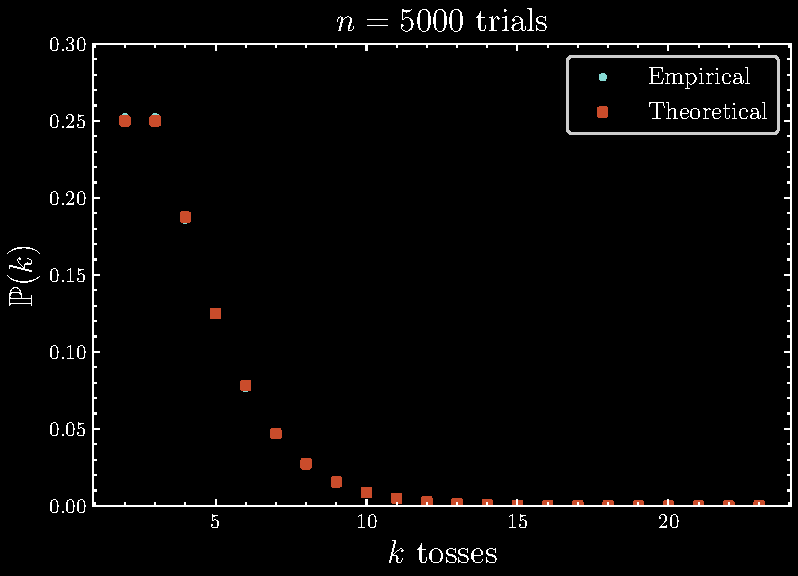
\includegraphics[width=1.0\textwidth]{chap1/chap1ex5.eps}
\end{center}

When we simulate the experiment for a large number of trials, we can see that the empirical results are quite close to the expected theoretical outcomes.

\newpage
% QUESTION 6
\qs{1.10.6}{Let \(\Omega = \{0, 1, \dots, \} \). Prove that there does not exist a uniform distribution on \(\Omega\) (i.e., if \(\Prob(A) = \Prob(B)\) whenever \(\abs{A} = \abs{B}\), then \(\Prob\) cannot satisfy the axioms of probability).}

\begin{proof}[Proof] 
	Suppose that \(\Omega\) has a uniform distribution, and \(\Prob(A) = \Prob(B)\) whenever \(\abs{A} = \abs{B}\). Consider the disjoint singletons \(\{0\}, \{1\}, \dots\). By Axiom 3, we have
	\[
	\Prob\left(\bigcup_{k=0}^{\infty} \{k\} \right) = \sum_{k=0}^{\infty} \Prob(\{k\})
	\]
However,
\[
	\bigcup_{k=0}^{\infty} \{k\} = \Omega 
\]
which from Axiom 2 implies
\[
	\Prob\left(\bigcup_{k=0}^{\infty} \{k\} \right) = \Prob(\Omega) = 1
\]
But by our uniform distribution assumption, each constituent of the sum of singleton probabilities is zero (picking a particular integer out of infinite possibilities is effectively zero probability). Thus we must have
\[
	\sum_{k=0}^{\infty} \Prob(\{k\}) = 0
\]
But \(\Prob\big(\bigcup_{k=0}^{\infty} \{k\} \big) = 1 \), a contradiction.
\end{proof}

% QUESTION 7
\qs{1.10.7}{Let \(A_{1}, A_{2},\dots\) be events. Show that
\[
	\Prob\left(\bigcup_{n=1}^{\infty} A_{n} \right) \le \sum_{n=1}^{\infty} \Prob(A_{n}).
\]
Hint: Define \(B_{n} = A_{n} - \bigcup_{i=1}^{n-1} A_{i} \). Then show that the \(B_{n}\) are disjoint and that \(\bigcup_{n=1}^{\infty} A_{n} = \bigcup_{n=1}^{\infty} B_{n} \). 
}
\begin{proof}[Proof] 
	Define \(B_{n} = A_{n} - \bigcup_{i=1}^{n-1} A_{i} \). First we prove the \(B_{n}\) are disjoint. Take \(B_{k}, B_{j}\) for \(k \neq j\). Without loss of generality, suppose \(k < j\). Let \(\omega \in B_{k}\). Then \(\omega \in A_{k} - \bigcup_{i=1}^{k-1} A_{i} \); importantly, \(\omega \in A_{k}\). Then we must have \(\omega \in \bigcup_{i=1}^{j-1} A_{i} \), implying \(\omega \not\in A_{j} - \bigcup_{i=1}^{j-1} A_{i} = B_{j} \).

	Conversely, if \(\omega \in B_{j} = A_{j} - \bigcup_{i=1}^{j-1} A_{i} \), we must have \(\omega \not\in \bigcup_{i=1}^{j-1} A_{i}\). Then we have \(\omega \not\in A_{k}\), implying \(\omega \not\in A_{k} - \bigcup_{i=1}^{k-1} A_{i} \). Thus \(B_{i} \cap B_{j} = \varnothing\) and \(B_{i}, B_{j}\) are disjoint.

	Now, we establish \(\bigcup_{n=1}^{\infty} A_{n} = \bigcup_{n=1}^{\infty} B_{n} \). Let \(\omega \in \bigcup_{n=1}^{\infty} \). Then \(\omega \in A_{k}\) for some \(k\)('s). Choose the \(A_{k}\) with the lowest \(k\). Then \(\omega \in A_{k} - \bigcup_{i=1}^{k-1} A_{i} = B_{k} \) implies \(\omega \in \bigcup_{n=1}^{\infty} B_{n} \).

	Conversely, let \(\omega \in \bigcup_{n=1}^{\infty} B_{n} \). Then \(\omega \in B_{k} = A_{k} - \bigcup_{i=1}^{k=1} A_{i} \) for some \(k\)('s). Then \(\omega \in A_{k}\) implies \(\omega \in \bigcup_{n=1}^{\infty} A_{n} \). Thus \(\bigcup_{n=1}^{\infty} A_{n} = \bigcup_{n=1}^{\infty} B_{n}  \).

	By Axiom 3 and the disjointness of \(B_{n}\), we have
\[
	\Prob\left(\bigcup_{n=1}^{\infty} B_{n} \right) = \sum_{n=1}^{\infty} \Prob(B_{n})
\]
Since \(B_{n} = A_{n} - \bigcup_{i=1}^{n-1} A_{i} \subset A_{n} \), we have \(\Prob(B_{n}) \le \Prob(A_{n})\) for all \(n\). Then \(\sum_{n=1}^{\infty} \Prob(B_{n}) \le \sum_{n=1}^{\infty} \Prob(A_{n})\). At last we may conclude
\[
	\Prob\left(\bigcup_{n=1}^{\infty} A_{n}  \right) \le \sum_{n=1}^{\infty} \Prob(A_{n})
\]
\end{proof}

% QUESTION 8
\qs{1.10.8}{Suppose that \(\Prob(A_{i}) = 1\) for each \(i\). Prove that
\[
	\Prob\left(\bigcap_{i=1}^{\infty}A_{i} \right) = 1
\]
}

\begin{proof}[Proof] 
	By premise, \(\Prob(A_{i} = 1)\) implies \(\Prob(A_{i}^{c}) = 1 - \Prob(A_{i}) = 0\). Now, since \(A_{1}^{c}, A_{2}^{c},\dots\) all have probability zero, it must be the case that \(\Prob(\bigcup_{i=1}^{\infty}A_{i}^{c} ) = 0\). By De Morgan's laws,
\[
	\Prob\left(\bigcup_{i=1}^{\infty} A_{i}^{c} \right) = \Prob\left( \left(\bigcap_{i=1}^{\infty} A_{i} \right)^{c} \right) = 0 
\]
Allowing us to conclude
\[
	\Prob\left( \bigcap_{i=1}^{\infty} A_{i} \right) = 1 - \Prob\left( \left(\bigcap_{i=1}^{\infty} A_{i} \right)^{c} \right) = 1 
\]
\end{proof}

% QUESTION 9
\qs{1.10.9}{For fixed \(B\) such that \(\Prob(B) > 0\), show that \(\Prob(\cdot \mid B)\) satifies the axioms of probability.}

\begin{proof}[Proof] 
(i) For independent \(\cdot, B\), we have \(\Prob(\cdot B) = \Prob(\cdot) \Prob(B)\), and if \(\Prob(\cdot) \ge 0\) then \(\Prob(\cdot \mid B) = \Prob(\cdot) \ge 0\). Otherwise, \(\Prob(\cdot B), \Prob(B) \ge 0\) implies \(\Prob(\cdot \mid B) \ge 0\).
\vspace{12pt}
\par (ii) If \(\cdot = \Omega\), then
\[
	\Prob(\Omega \mid B) = \frac{\Prob(\Omega B)}{\Prob(B)} = \frac{\Prob(\Omega) \Prob(B)}{\Prob(B)} = \Prob(\Omega) = 1
\]
\vspace{12pt}
\par (iii) If \(A_{i} \cap A_{j} = \varnothing\), then \( (A_{i} \cap B) \cap (A_{j} \cap B) = \varnothing\). Then we have

\begin{align*}
	\Prob(A_{i} \cup A_{j} \mid B) & = \frac{\Prob((A_{i} \cup A_{j}) \cap B)}{\Prob(B)} \\
			       & = \frac{\Prob((A_{i} \cap B) \cup (A_{j} \cap B))}{\Prob(B)}  \\
			       & = \frac{\Prob(A_{i} \cap B) + \Prob(A_{j} \cap B)}{\Prob(B)} \\
			       & = \Prob(A_{i} \mid B) + \Prob(A_{j} \mid B)
\end{align*}

To generalize for infinitely many disjoint events \(A_{i}\), observe that 
\[
	\left( \bigcup_{i = 1}^{\infty} A_{i} \right) \cap B = \bigcup_{i = 1}^{\infty} (A_{i} \cap B)
\]
Applying the logic for the case with two disjoint events, we can immediately conclude
\[
	\Prob\left( \bigcup_{i = 1}^{\infty} A_{i} \Bigg| B \right) = \sum_{i=1}^{\infty} \Prob(A_{i} \mid B)
\]
\end{proof}

\newpage
% QUESTION 10
\qs{1.10.10}{You have probably heard it before. Now you can solve it rigorously. It is called the "Monty Hall Problem." A prize is placed at random behind one of three doors. You pick a door. To be concrete, let's suppose you always pick door 1. Now Monty Hall chooses one of the other two doors, opens it and shows you that it is empty. He then gives you the opportunity to keep your door or switch to the other unopened door. Should you stay or switch? Intuition suggests it doesn't matter. The correct answer is you should switch. Prove it. It will  help to specify the sample space and the relevant events carefully. Thus write \(\Omega = \left\{\, (\omega_{1}, \omega_{2}) \colon \omega_{i} \in \{1,2,3 \} \,\right\}\) where \(\omega_{1}\) is where the prize is and \(\omega_{2}\) is the door Monty opens. }

There are some insights we should be aware of. Firstly, there is equal chance of the prize appearing behind any one of the three doors, i.e., \(\Prob(\text{Prize, Door } i) = 1/3\). Secondly, the choice of door for Monty Hall \textit{depends on our choice of door}. Our pick of door also follows equal probability for each door, or \(1/3\).

Using Bayes' Theorem, without loss of generality, suppose you pick door 1, the prize lies behind door 2, and Monty Hall picks door 3. We wish to find the probability that the prize is behind door 2, \textit{given that Monty Hall opens door 3}.
\begin{align*}
	\Prob(\text{Prize, Door }2 \mid \text{Monty, Door }3) & = \frac{\Prob(\text{M, D }3 \mid \text{P, D } 2)\Prob(\text{P, D }2)}{\sum \Prob(\text{M, D } 3 \mid \text{P, D } i)\Prob(\text{P, D } i)} \\
	 & = \frac{1 \cdot 1/3}{1 \cdot 1/3 + 1/2 \cdot 1/3 + 0 \cdot 1/3} \\
	 & = \boxed{2/3}
\end{align*}

Here, it is advantageous to switch doors, as the prior probability \((1/3)\) changes to the posterior probability \((2/3)\) once Monty Hall diverges additional information that his door is empty.

It is useful to illustrate the sample space by way of a probability tree:

\begin{center}
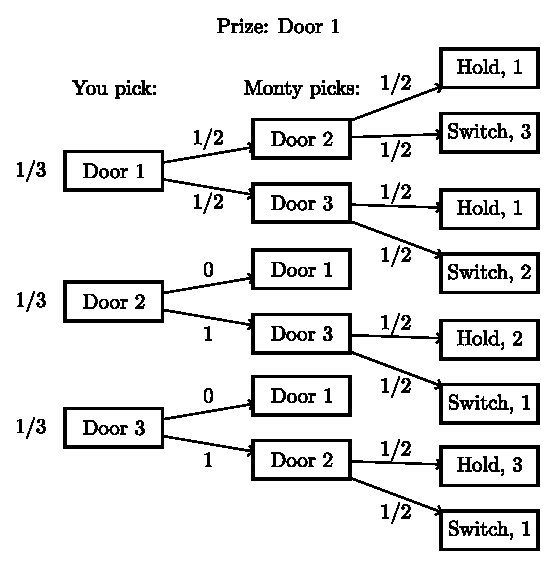
\includegraphics[width=1.0\textwidth]{chap1/c1q10.eps}
\end{center}

Assuming without loss of generality that the prize lies behind door 1, we can calculate the conditional probabilities of winning given that we either hold or switch. 

Let \(Y\) be your choice of door and \(M\) be Monty Hall's. Moreover, let \(\alpha\) be
\begin{align*}
	\alpha & = \Prob(Y=1)\Prob(M=2 \mid Y=1)\Prob(\text{Hold }1 \mid M = 2) \\ 
	 & \quad + \Prob(Y=1)\Prob(M=3 \mid Y=1)\Prob(\text{Hold }1 \mid M=3) \\
	 & \quad + \Prob(Y=2)\Prob(M=3 \mid Y=2)\Prob(\text{Hold }2 \mid M=3) \\
	 & \quad + \Prob(Y=3)\Prob(M=2 \mid Y=3)\Prob(\text{Hold } 3 \mid M=2) \\
	 & = 1/3 \cdot 1/2 \cdot 1/2 + 1/3 \cdot 1/2 \cdot 1/2 + 1/3 \cdot 1/2 + 1/3 \cdot 1/2 \\
	 & = 1/2
\end{align*}

We calculate
\begin{align*}
	\Prob(\text{Win } \mid \text{ Hold}) & = \frac{\Prob(Y=1)\Prob(M=2 \mid Y=1)\Prob(\text{Hold } 1 \mid M=2)}{\alpha} \\
	 & \quad + \frac{\Prob(Y=1)\Prob(M=3 \mid Y=1)\Prob(\text{Hold }1 \mid M=3)}{\alpha} \\
	 & = \frac{1/3 \cdot 1/2 \cdot 1/2 + 1/3 \cdot 1/2 \cdot 1/2}{1/2} \\
	 & = \boxed{1/3}
\end{align*}

An analogous calculation for the switching conditional probability gives us
\[
	\Prob(\text{Win } \mid \text{ Switch}) = \boxed{2/3}
\]
Lastly, there is a famous anecdote of Erd{\"o}s refusing to accept the result of the Monty Hall problem until examining a simulation of the game. You may find yourself burdened by a similar sentiment. Indeed, the experimental result aligns with our derivations above:

\begin{center}
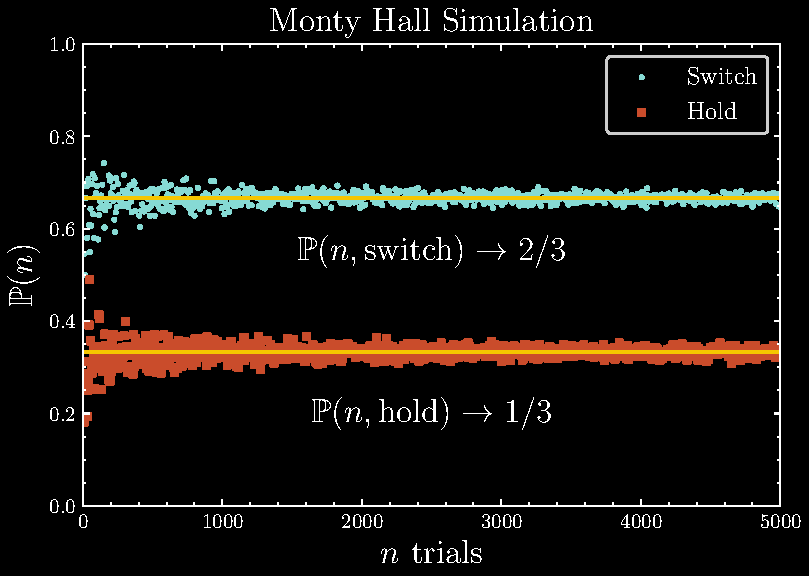
\includegraphics[width=1.0\textwidth]{chap1/chap1ex10.eps}
\end{center}

% QUESTION 11
\qs{1.10.11}{Suppose that \(A\) and \(B\) are independent events. Show that \(A^{c}\) and \(B^{c}\) are independent events.}

\begin{proof}[Proof] 
By premise, \(\Prob(AB) = \Prob(A)\Prob(B)\). We have \(\Prob(A^{c}) = 1 - \Prob(A)\) and \(\Prob(B^{c}) = 1 - \Prob(B)\). To find \(\Prob(A^{c} B ^{c})\), we observe these disjoint events:

\begin{align*}
	\Prob(A-B) & = \Prob(A) - \Prob(AB) \\
	\Prob(B-A) & = \Prob(B) - \Prob(AB) \\
	           & \Prob(AB) \\
		   & \Prob(A^{c}B^{c})
\end{align*}

Thus we have
\[
	1 = \Prob(A-B) + \Prob(B-A) + \Prob(AB) + \Prob(A^{c}B^{c})
\]
which implies
\begin{align*}
	\Prob(A^{c}B^{c}) & = 1 - \Prob(A-B) - \Prob(B-A) - \Prob(AB) \\
	 & = 1 - (\Prob(A) - \Prob(AB)) - (\Prob(B) - \Prob(AB)) - \Prob(AB) \\
	 & = 1 - \Prob(A) - \Prob(B) + \Prob(AB)
\end{align*}
Now calculate
\begin{align*}
	\Prob(A^{c})\Prob(B^{c}) & = (1 - \Prob(A))(1 - \Prob(B)) \\
	 & = 1 - \Prob(A) - \Prob(B) + \Prob(A)\Prob(B) \\
	 & = 1 - \Prob(A) - \Prob(B) + \Prob(AB)
\end{align*}
Thus \(\Prob(A^{c}B^{c}) = \Prob(A^{c})\Prob(B^{c})\), and \(A^{c}\) and \(B^{c}\) are independent.
\end{proof}

% QUESTION 12
\qs{1.10.12}{There are three cards. The first is green on both sides, the second is red on both sides and the third is green on one side and red on the other. We choose a card at random and we see one side (also chosen at random). If the side we see is green, what is the probability that the other side is also green? Many people intuitively answer \(1/2\). Show that the correct answer is \(2/3\).}
\begin{proof}[Proof] 
Let \(GG, RR, GR\) correspond to the first, second, and third cards. Using Bayes' Theorem: we calculate the probability of having drawn a \(GG\) card given that we see \(G\), or \(GR\) given that we see \(G\). Calculate
\begin{align*}
	\Prob(GG \mid G) & = \frac{\Prob(G \mid GG) \Prob(GG)}{\Prob(G \mid GG)\Prob(GG) + \Prob(G \mid RR)\Prob(RR) + \Prob(G \mid GR)\Prob(GR)} \\
	 & = \frac{1 \cdot 1/3}{1 \cdot 1/3 + 0 \cdot 1/3 + 1/2 \cdot 1/3} \\
	 & = \boxed{2/3} \\
	\Prob(GR \mid G) & = \frac{\Prob(G \mid GR)\Prob(GR)}{\Prob(G \mid GR)\Prob(GR) + \Prob(G \mid RR)\Prob(RR) + \Prob(G \mid GG)\Prob(GG)} \\
	 & = \frac{1/2 \cdot 1/3}{1/2 \cdot 1/3 + 0 \cdot 1/3 + 1 \cdot 1/3} \\
	 & = \boxed{1/3}
\end{align*}
\end{proof}

Simulating the card game, we find that the empirical outcome agrees with our theoretical result.

\begin{center}
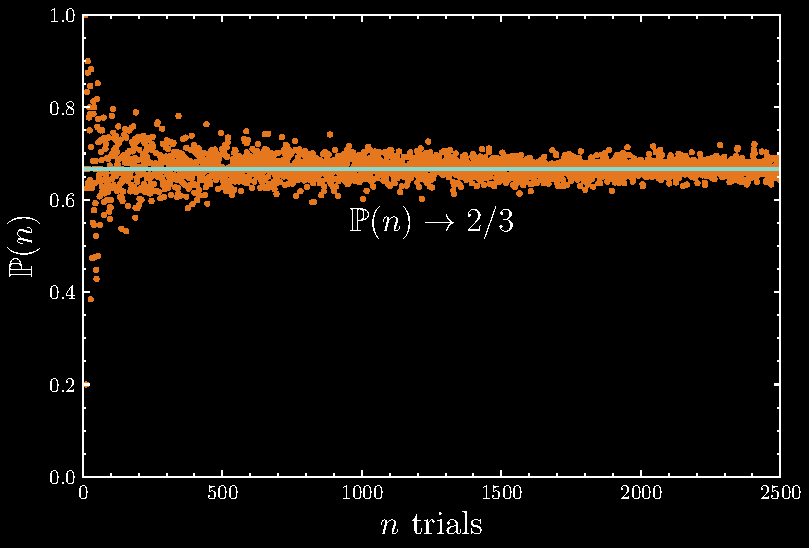
\includegraphics[width=1.0\textwidth]{chap1/chap1ex12}
\end{center}

% QUESTION 13
\qs{1.10.13}{Suppose that a fair coin is tossed repeatedly until both a head and tail have appeared at least once.
\begin{enumerate}[label=(\alph*)]
	\item Describe the sample space \(\Omega\).
	\item What is the probability that three tosses will be required?
\end{enumerate}}

(a) The sample space is given by
\[
	\Omega = \{HT, HHT, \dots, \underbrace{H \cdots H}_{k}T, \dots, TH, TTH, \dots, \underbrace{T \cdots T}_{k}H, \dots \}
\]
\vspace{12pt}
\par (b) The theoretical derivation of the probability is
\begin{align*}
	\Prob(\text{3 tosses}) & = \Prob(HHT) + \Prob(TTH)  \\
	 & = (1/2)^{3} + (1/2)^{3} \\
	 & = \boxed{1/4}
\end{align*}

By simulation, we can observe the empirical probability of three tosses aligns with the theoretical result, as well as the probabilities for other numbers of tosses:

\begin{center}
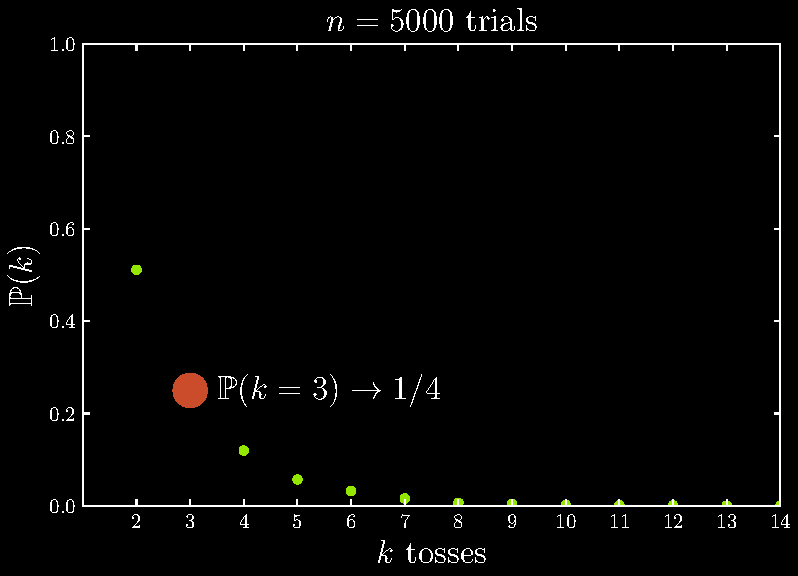
\includegraphics[width=1.0\textwidth]{chap1/chap1ex13}
\end{center}

% QUESTION 14
\qs{1.10.14}{Show that if \(\Prob(A) = 0\) or \(\Prob(A) = 1\) then \(A\) is independent of every other event. Show that if \(A\) is independent of itself then \(\Prob(A)\) is either \(0\) or \(1\).}
\begin{proof}[Proof] 
Let \(B\) be any event. Then if \(\Prob(A) = 0\), we have \(\Prob(AB) = 0\). Put differently, if \(A\) can never happen, then surely \(A\) \textit{and} \(B\) could never happen. Now, it must also be true that \(P(A)\Prob(B) = 0\), so it follows that \(\Prob(AB) = \Prob(A)\Prob(B) = 0\) and \(A\) is independent of all events.

Now suppose \(\Prob(A) = 1\). Then \(\Prob(AB) = \Prob(B)\). The reasoning is that since \(A\) will \textit{always} happen, whether \(A\) and \(B\) happen together is contingent on \(B\) happening. Thus we can write \(\Prob(AB) = \Prob(A)\Prob(B) = \Prob(B)\), again proving independence of A relative to all other events.

Lastly, suppose \(A\) is independent of itself. Then \(\Prob(AA) = \Prob(A) = \Prob(A)\Prob(A)\), implying \(\Prob(A) = 0\) or \(\Prob(A) = 1\).
\end{proof}

\newpage
% QUESTION 15
\qs{1.10.15}{The probability that a child has blue eyes is \(1/4\). Assume independence between children. Consider a family with \(3\) children.\begin{enumerate}[label=(\alph*)]
	\item If it is known that at least one child has blue eyes, what is the probability that at least two children have blue eyes?
	\item If it is known that the youngest child has blue eyes, what is the probability that at least two children have blue eyes?
\end{enumerate}}

(a) The complement event to "at least one child has blue eyes" -- call it \(A\) -- is "no child has blue eyes." The probability that a child does not have blue eyes is \(1 - p = 3/4\). Then we have
\[
	\Prob(A) = 1 - (3/4)^{3} = 1 - 27/64 = 37/64
\]
The probability that "at least two children have blue eyes" -- call this one \(B\) -- is the sum of the mutually exclusive probabilities of either two or three children having blue eyes. This is given by
\begin{align*}
	\Prob(B) & = \Prob(\text{2 children} + \text{3 children}) \\
		 & = \binom{3}{2} (1/4)^{2} (3/4) + (1/4)^{3} \\
		 & = 9/64 + 1/64 \\
		 & = 10/64
\end{align*}
Now we can calculate the probability of at least two children having blue eyes, given that at least one child has blue eyes.
\begin{align*}
	\Prob(B \mid A) & = \frac{\Prob(BA)}{\Prob(A)} \\
	 & = (10/64)(64/37) \\
	 & = \boxed{10/37}
\end{align*}
\par (b) The probability that the youngest child has blue eyes (call it C) is \(1/4\). Let \(D\) be the event that at least two children have blue eyes, with one of them being the youngest child. Then we have
\begin{align*}
	\Prob(D) & = 2(1/4)^{2}(3/4) + (1/4)^{3} \\
	 & = 6/64 + 1/64 \\
         & = 7/64
\end{align*}
Lastly, the probability that at least two children have blue eyes given that the youngest child is known to have blue eyes is
\begin{align*}
	\Prob(D \mid C) & = \frac{\Prob(DC)}{\Prob(C)} \\
	 & = \frac{7/64}{1/4} \\
	 & = \boxed{7/16}
\end{align*}

% QUESTION 16
\qs{1.10.16}{Prove Lemma 1.14.}
\lemma{(Wasserman 1.14)}{If \(A\) and \(B\) are independent events then \(\Prob(A \mid B) = \Prob(A)\). Also, for any pair of events \(A\) and \(B\),\[
	\Prob(AB) = \Prob(A \mid B)\Prob(B) = \Prob(B \mid A)\Prob(A)
\]}
\begin{proof}[Proof] 
\begin{align*}
	\Prob(A \mid B) = \frac{\Prob(AB)}{\Prob(B)} & = \frac{\Prob(A)\Prob(B)}{\Prob(B)} = \Prob(A) \\
	\Prob(A \mid B) = \frac{\Prob(AB)}{\Prob(B)} & \implies \Prob(A \mid B) \Prob(B) = \Prob(AB)  \\
	\Prob(B \mid A) = \frac{\Prob(AB)}{\Prob(A)} & \implies \Prob(B \mid A)\Prob(A) = \Prob(AB)
\end{align*}
\end{proof}

% QUESTION 17
\qs{1.10.17}{Show that
\[
	\Prob(ABC) = \Prob(A \mid BC)\Prob(B \mid C)\Prob(C)
\]}
\begin{proof}[Proof] 
\[
	\Prob(ABC) = \Prob(A  \mid  BC)\Prob(BC) = \Prob(A \mid BC)\Prob(B \mid C)\Prob(C)
\]
\end{proof}

% QUESTION 18
\qs{1.10.18}{Suppose \(k\) events form a partition of the sample space \(\Omega\), i.e., they are disjoint and \(\bigcup_{i=1}^{k} A_{i} = \Omega \). Assume that \(\Prob(B) > 0\). Prove that if \(\Prob(A_{1}  \mid  B) < \Prob(A_{1})\) then \(\Prob(A_{i}  \mid  B) > \Prob(A_{i})\) for some \(i = 2, \dots, k\).}
\begin{proof}[Proof] 
By disjointness of events, we have
\[
	\sum_{i=1}^{k} \Prob(A_{i}) = 1 \quad \text{and} \quad \sum_{i=1}^{k} \Prob(A_{i}  \mid  B) = 1
\]
with the second equality following from 1.10.9. Let \(\Prob(A_{1}  \mid  B) < \Prob(A_{1})\). It cannot be the case that we have \(\Prob(A_{i}  \mid  B) < \Prob(A_{i})\) for the remaining \(i = 2,\dots,k\), for this would violate additivity of the conditional probabilities to unity:
\[
	\sum_{i=2}^{k} \Prob(A_{i}  \mid  B) < \sum_{i=2}^{k} \Prob(A_{i}) = 1
\]
So would the condition that \(\Prob(A_{i}  \mid  B) = \Prob(A_{i})\) for the remaining \(i\). Thus at least one of the \(\Prob(A_{i}  \mid  B)\) must be greater than \(A_{i}\) for the unity sum condition to be met.
\end{proof}

% QUESTION 19
\qs{1.10.19}{Suppose that 30 percent of computer owners use a Macintosh, 50 percent use Windows, and 20 percent use Linux. Suppose that 65 percent of the Mac users have succumbed to a computer virus, 82 percent of the Windows users get the virus, and 50 percent of the Linux users get the virus. We select a person at random and learn that her system was infected with the virus. What is the probability that she is a Windows user?}

By Bayes' Theorem:
\begin{align*}
	\Prob(\text{Windows}  \mid  \text{Virus}) & = \frac{\Prob(\text{V}  \mid  \text{W})\Prob(\text{W})}{\Prob(\text{V}  \mid  \text{W})\Prob(\text{W}) + \Prob(\text{V}  \mid  \text{M})\Prob(\text{M}) + \Prob(\text{V}  \mid  \text{L})\Prob(\text{L})}  \\
	 & = \frac{0.82 \cdot 0.5}{0.82 \cdot 0.5 + 0.65 \cdot 0.3 + 0.5 \cdot 0.2} \\
	 & = \boxed{0.582}
\end{align*}

% QUESTION 20
\qs{1.10.20}{A box contains 5 coins and each has a different probability of showing heads. Let \(p_{1}, \dots, p_{5}\) denote the probability of heads on each coin. Suppose that
\[
	p_{1} = 0, p_{2} = 1/4, p_{3} = 1/2, p_{4} = 3/4 \ \text{and} \ p_{5} = 1.
\]
Let \(H\) denote "heads is obtained" and let \(C_{i}\) denote the event that coin \(i\) is selected.
\begin{enumerate}[label=(\alph*)]
	\item Select a coin at random and toss it. Suppose a head is obtained. What is the posterior probability that coin \(i\) was selected \((i = 1,\dots,5)\)? In other words, find \(\Prob(C_{i} \mid H)\) for \(i = 1,\dots,5\).
	\item Toss the coin again. What is the probability of another head? In other words find \(\Prob(H_{2} \mid H_{1})\) where \(H_{j} = \text{"heads on toss } j.\)" 

	Now suppose that the experiment was carried out as follows: We select a coin at random and toss it until a head is obtained.
	\item Find \(\Prob(C_{i} \mid B_{4})\) where \(B_{4} = \) "first head is obtained in toss 4."
\end{enumerate}
}	

Apply Bayes' Theorem for all parts.

(a) Here, \(\sum \Prob(H \mid C_{i})\Prob(C_{i}) = 1/5 \cdot \Big(\sum p_{i} \Big) = 1/5 \cdot 5/2 = 1/2 \).

\begin{align*}
	\Prob(C_{1} \mid H) & = \frac{\Prob(H \mid C_{1})\Prob(C_{1})}{\sum \Prob(H \mid C_{i})\Prob(C_{i})} = \boxed{0} \\
	\Prob(C_{2} \mid H) & = \frac{\Prob(H \mid C_{2})\Prob(C_{2})}{\sum \Prob(H \mid C_{i})\Prob(C_{i})} = \frac{1/4 \cdot 1/5}{1/2} = \boxed{1/10}  \\
	\Prob(C_{3} \mid H) & = \frac{\Prob(H \mid C_{3})\Prob(C_{3})}{\sum \Prob(H \mid C_{i})\Prob(C_{i})} = \frac{1/2 \cdot 1/5}{1/2} = \boxed{2/10} \\
	\Prob(C_{4} \mid H) & = \frac{\Prob(H \mid C_{4})\Prob(C_{4})}{\sum \Prob(H \mid C_{i})\Prob(C_{i})} = \frac{3/4 \cdot 1/5}{1/2} = \boxed{3/10} \\
	\Prob(C_{5} \mid H) & = \frac{\Prob(H \mid C_{5})\Prob(C_{5})}{\sum \Prob(H \mid C_{i})\Prob(C_{i})} = \frac{1 \cdot 1/5}{1/2} = \boxed{4/10}
\end{align*}

Empirical simulation:

\begin{center}
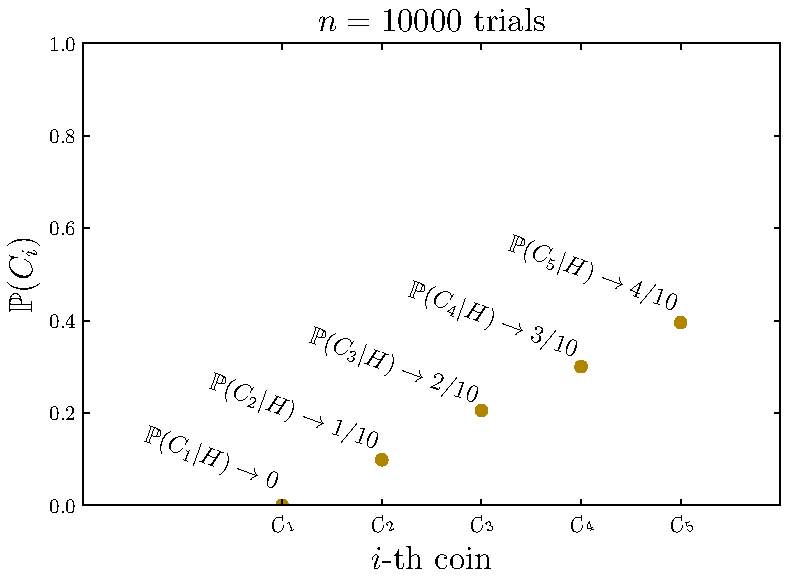
\includegraphics[width=1.0\textwidth]{chap1/chap1ex20a}
\end{center}

\par (b) By the Law of Total Probability, \(\Prob(H_{1}) = 1/5 \cdot \sum p_{i} = 1/2\). To calculate \(\Prob(H_{2} \mid H_{1})\), write
\begin{align*}
	\Prob(H_{2} \mid H_{1}) & = \frac{\Prob(H_{2}H_{1})}{\Prob(H_{1})} \\
	 & = \frac{1/5 \cdot \sum p_{i}^{2}}{1/2} \\
	 & = \frac{3/8}{1/2} \\
	 & = \boxed{3/4}
\end{align*}

Empirical simulation:

\begin{center}
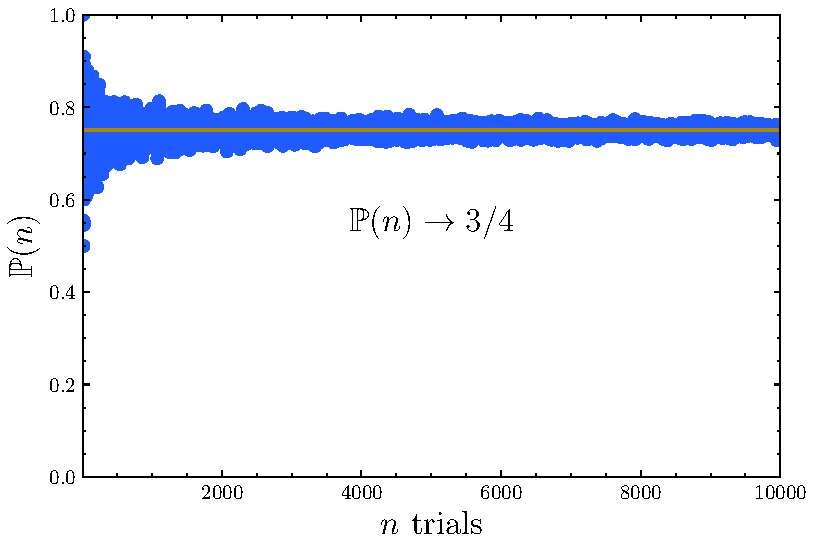
\includegraphics[width=1.0\textwidth]{chap1/chap1ex20b}
\end{center}

\par (c) Here, \(\sum \Prob(B_{4} \mid C_{i})\Prob(C_{i}) = 1/5 \cdot \sum (1-p_{i})^{3}p_{i} = 0.0359375\).

\begin{align*}
	\Prob(C_{1} \mid B_{4}) & = \frac{\Prob(B_{4} \mid C_{1})\Prob(C_{1})}{\sum \Prob(B_{4} \mid C_{i})\Prob(C_{i})} = \boxed{0}  \\
\Prob(C_{2} \mid B_{4}) & = \frac{\Prob(B_{4} \mid C_{2})\Prob(C_{2})}{\sum \Prob(B_{4} \mid C_{i})\Prob(C_{i})} = \frac{(3/4)^{3}(1/4)(1/5)}{0.0359375} = \boxed{0.587} \\
	\Prob(C_{3} \mid B_{4}) & = \frac{\Prob(B_{4} \mid C_{3})\Prob(C_{3})}{\sum \Prob(B_{4} \mid C_{i})\Prob(C_{i})} = \frac{(1/2)^{4}(1/5)}{0.0359375} = \boxed{0.348} \\
	\Prob(C_{4} \mid B_{4}) & = \frac{\Prob(B_{4} \mid C_{4})\Prob(C_{4})}{\sum \Prob(B_{4} \mid C_{i})\Prob(C_{i})} = \frac{(1/4)^{3}(3/4)(1/5)}{0.0359375} = \boxed{0.065} \\
	\Prob(C_{5} \mid B_{4}) & = \frac{\Prob(B_{4} \mid C_{5})\Prob(C_{5})}{\sum \Prob(B_{4} \mid C_{i})\Prob(C_{i})} = \boxed{0}
\end{align*}

Empirical simulation:

\begin{center}
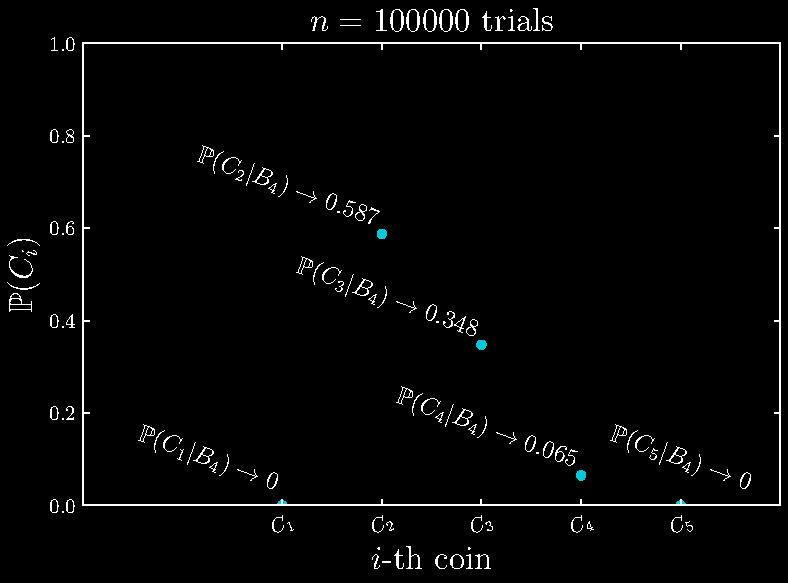
\includegraphics[width=1.0\textwidth]{chap1/chap1ex20c}
\end{center}

% QUESTION 21
\qs{1.10.21}{\textsf{(Computer Experiment.)} Suppose a coin has probability \(p\) of falling heads up. If we flip the coin many times, we would expect the proportion of heads to be near \(p\). We will make this formal later. Take \(p = .3\) and \(n = 1,000\) and simulate \(n\) coin flips. Plot the proportion of heads as a function of \(n\). Repeat for \(p = .03\).}

As intuitively anticipated, for large \(n\), the probability of heads tends towards \(0.3\) or \(0.03\).

\begin{center}
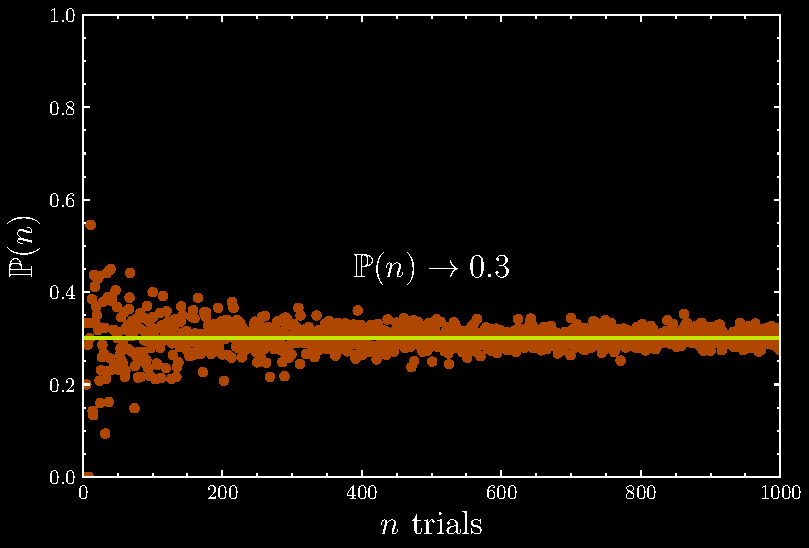
\includegraphics[width=1.0\textwidth]{chap1/chap1ex21i.eps}
\end{center}

\begin{center}
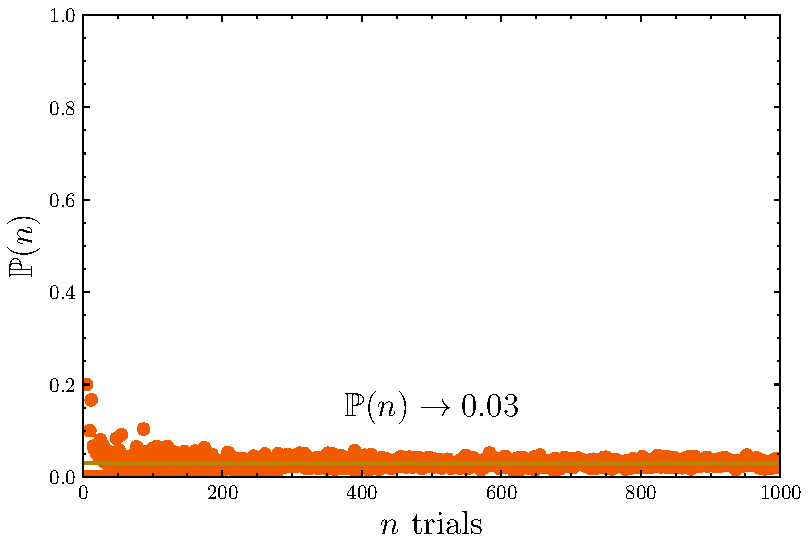
\includegraphics[width=1.0\textwidth]{chap1/chap1ex21ii.eps}
\end{center}

% QUESTION 22
\qs{1.10.22}{\textsf{(Computer Experiment.)} Suppose we flip a coin \(n\) times and let \(p\) denote the probability of heads. Let \(X\) be the number of heads. We call \(X\) a binomial random variable, which is discussed in the next chapter. Intuition suggests that \(X\) will be close to \(np\). To see if this is true, we can repeat this experiment many times and average the \(X\) values. Carry out a simulation and compare the average of the \(X\)'s to \(np\). Try this for \(p = .3\) and \(n = 10, n = 100\), and \(n = 1,000\).}

We run 1,000 trials for 10, 100, and 1,000 flips. The average number of heads for each number of flips are 3.009, 30.13, and 299.746, compared to \(np =\) 3, 30, and 300.

% QUESTION 23
\qs{1.10.23}{\textsf{(Computer Experiment.)} Here we will get some experience simulating conditional probabilities. Consider tossing a fair die. Let \(A = \{2,4,6 \}\) and \(B = \{1,2,3,4 \} \). Then, \(\Prob(A) = 1/2, \Prob(B) = 2/3\) and \(\Prob(AB) = 1/3\). Since \(\Prob(AB) = \Prob(A)\Prob(B)\), the events \(A\) and \(B\) are independent. Simulate draws from the sample space and verify that \(\widehat{\Prob}(AB) = \widehat{\Prob}(A)\widehat{\Prob}(B)\) where \(\widehat{\Prob}(A)\) is the proportion of times \(A\) occurred in the simulation and similarly for \(\widehat{\Prob}(AB)\) and \(\widehat{\Prob}(B)\). Now find two events \(A\) and \(B\) that are not independent. Compute \(\widehat{\Prob}(A), \widehat{\Prob}(B)\) and \(\widehat{\Prob}(AB)\). Compare the calculated values to their theoretical values. Report your results and interpret. }

Now suppose we have $A = B = \{k\}$ where $k$ is any integer $1, \dots, 6$. Then $\mathbb{P}(A) = \mathbb{P}(B) = \mathbb{P}(AB) = 1/6$, but $\mathbb{P}(A)\mathbb{P}(B) = 1/36$. Thus $A$ and $B$ are not independent. In general, we can conclude that any event cannot be independent of itself unless the probability of the event is either 0 or 1.

\end{document}
